\documentclass{standalone}
\usepackage{tikz}
\usetikzlibrary{patterns, positioning}


\begin{document}
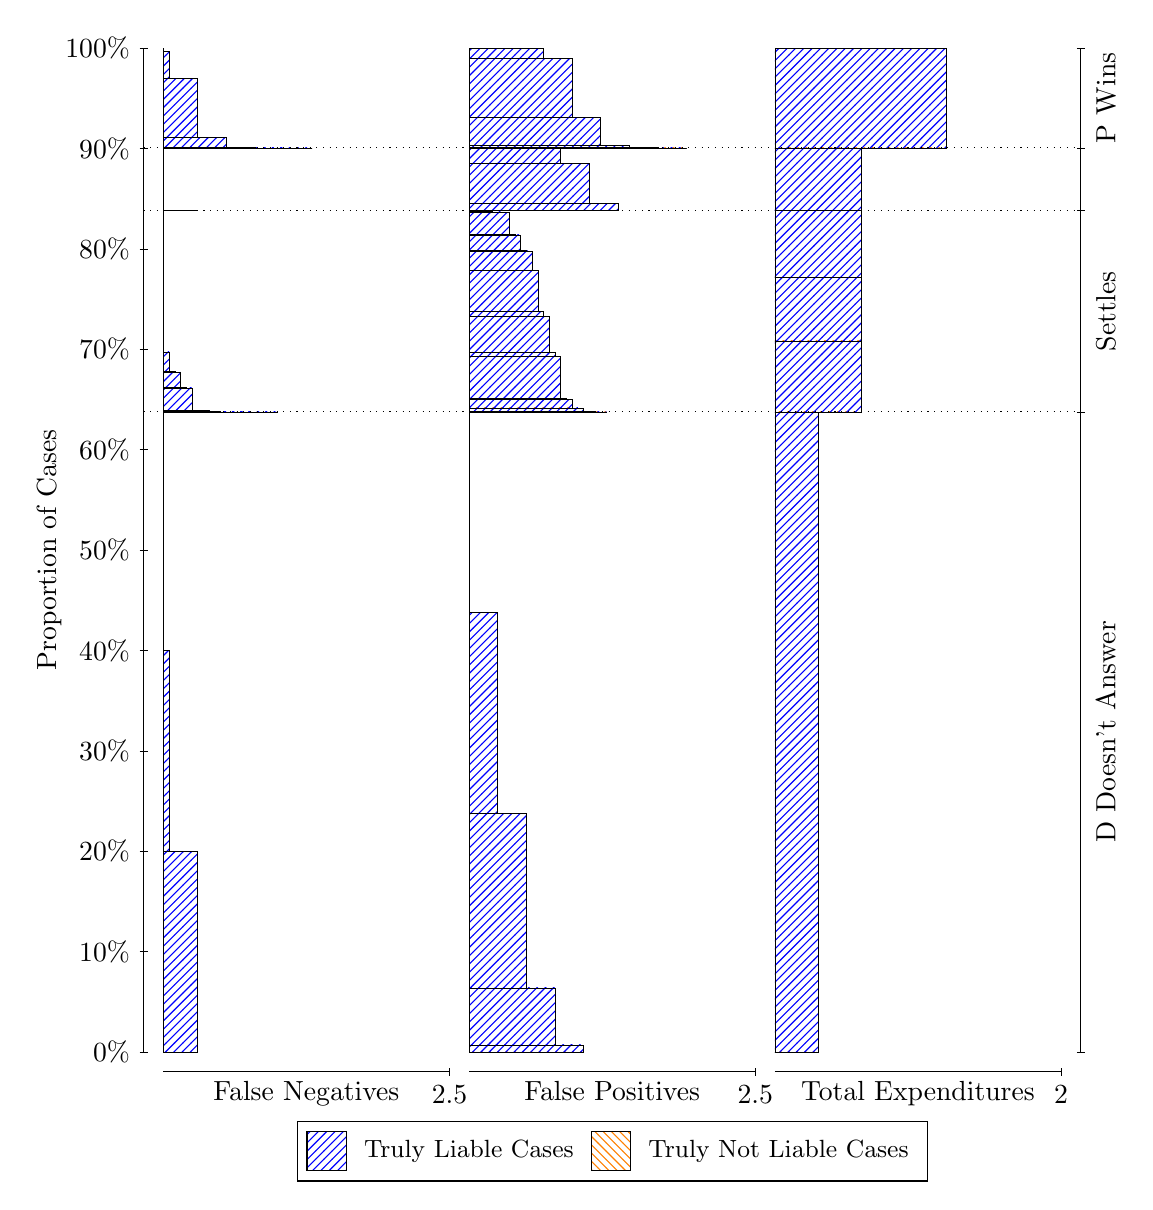
\begin{tikzpicture}
\draw[black, very thin] (1.5,1.75) -- (1.5,14.5);
\node[rotate=90, text=black, anchor=center] at (0.3, 8.125) {Proportion of Cases};
\draw[black, very thin] (1.45,1.75) -- (1.55,1.75);
\node[text=black, anchor=east] at (1.45, 1.75) {0\%};
\draw[black, very thin] (1.45,3.025) -- (1.55,3.025);
\node[text=black, anchor=east] at (1.45, 3.025) {10\%};
\draw[black, very thin] (1.45,4.3) -- (1.55,4.3);
\node[text=black, anchor=east] at (1.45, 4.3) {20\%};
\draw[black, very thin] (1.45,5.575) -- (1.55,5.575);
\node[text=black, anchor=east] at (1.45, 5.575) {30\%};
\draw[black, very thin] (1.45,6.85) -- (1.55,6.85);
\node[text=black, anchor=east] at (1.45, 6.85) {40\%};
\draw[black, very thin] (1.45,8.125) -- (1.55,8.125);
\node[text=black, anchor=east] at (1.45, 8.125) {50\%};
\draw[black, very thin] (1.45,9.4) -- (1.55,9.4);
\node[text=black, anchor=east] at (1.45, 9.4) {60\%};
\draw[black, very thin] (1.45,10.675) -- (1.55,10.675);
\node[text=black, anchor=east] at (1.45, 10.675) {70\%};
\draw[black, very thin] (1.45,11.95) -- (1.55,11.95);
\node[text=black, anchor=east] at (1.45, 11.95) {80\%};
\draw[black, very thin] (1.45,13.225) -- (1.55,13.225);
\node[text=black, anchor=east] at (1.45, 13.225) {90\%};
\draw[black, very thin] (1.45,14.5) -- (1.55,14.5);
\node[text=black, anchor=east] at (1.45, 14.5) {100\%};

\draw[black, very thin] (13.4,1.75) -- (13.4,14.5);
\draw[black, very thin] (13.35,1.75) -- (13.45,1.75);
\node[anchor=west] at (13.35, 1.75) {};
\draw[black, very thin] (13.35,9.8791) -- (13.45,9.8791);
\node[anchor=west] at (13.35, 9.8791) {};
\draw[black, very thin] (13.35,12.435) -- (13.45,12.435);
\node[anchor=west] at (13.35, 12.435) {};
\draw[black, very thin] (13.35,13.233) -- (13.45,13.233);
\node[anchor=west] at (13.35, 13.233) {};
\draw[black, very thin] (13.35,14.5) -- (13.45,14.5);
\node[anchor=west] at (13.35, 14.5) {};

\draw[black, very thin, pattern color=blue, pattern=north east lines] (1.75,1.75) rectangle (2.186,4.2999);
\draw[black, very thin, pattern color=blue, pattern=north east lines] (1.75,4.2999) rectangle (1.8227,6.8471);
\draw[black, very thin, pattern color=orange, pattern=north west lines] (1.75,6.8471) rectangle (1.75,6.8471);
\draw[black, very thin, pattern color=blue, pattern=north east lines] (1.75,6.8471) rectangle (1.75,9.8791);
\draw[black, very thin, pattern color=blue, pattern=north east lines] (1.75,9.8791) rectangle (3.2033,9.8791);
\draw[black, very thin, pattern color=blue, pattern=north east lines] (1.75,9.8791) rectangle (3.058,9.8791);
\draw[black, very thin, pattern color=blue, pattern=north east lines] (1.75,9.8791) rectangle (2.9127,9.8791);
\draw[black, very thin, pattern color=blue, pattern=north east lines] (1.75,9.8791) rectangle (2.84,9.8791);
\draw[black, very thin, pattern color=blue, pattern=north east lines] (1.75,9.8791) rectangle (2.7673,9.8791);
\draw[black, very thin, pattern color=blue, pattern=north east lines] (1.75,9.8791) rectangle (2.6947,9.8791);
\draw[black, very thin, pattern color=blue, pattern=north east lines] (1.75,9.8791) rectangle (2.622,9.8791);
\draw[black, very thin, pattern color=blue, pattern=north east lines] (1.75,9.8791) rectangle (2.5493,9.8791);
\draw[black, very thin, pattern color=blue, pattern=north east lines] (1.75,9.8791) rectangle (2.4767,9.8884);
\draw[black, very thin, pattern color=blue, pattern=north east lines] (1.75,9.8884) rectangle (2.404,9.8884);
\draw[black, very thin, pattern color=blue, pattern=north east lines] (1.75,9.8884) rectangle (2.3313,9.8944);
\draw[black, very thin, pattern color=blue, pattern=north east lines] (1.75,9.8944) rectangle (2.3313,9.8944);
\draw[black, very thin, pattern color=blue, pattern=north east lines] (1.75,9.8944) rectangle (2.2587,9.8944);
\draw[black, very thin, pattern color=blue, pattern=north east lines] (1.75,9.8944) rectangle (2.186,9.9021);
\draw[black, very thin, pattern color=blue, pattern=north east lines] (1.75,9.9021) rectangle (2.1133,10.185);
\draw[black, very thin, pattern color=blue, pattern=north east lines] (1.75,10.185) rectangle (2.0407,10.187);
\draw[black, very thin, pattern color=blue, pattern=north east lines] (1.75,10.187) rectangle (1.968,10.386);
\draw[black, very thin, pattern color=blue, pattern=north east lines] (1.75,10.386) rectangle (1.968,10.386);
\draw[black, very thin, pattern color=blue, pattern=north east lines] (1.75,10.386) rectangle (1.8953,10.391);
\draw[black, very thin, pattern color=blue, pattern=north east lines] (1.75,10.391) rectangle (1.8227,10.641);
\draw[black, very thin, pattern color=orange, pattern=north west lines] (1.75,10.641) rectangle (1.75,10.641);
\draw[black, very thin, pattern color=blue, pattern=north east lines] (1.75,10.641) rectangle (1.75,12.435);
\draw[black, very thin, pattern color=blue, pattern=north east lines] (1.75,12.435) rectangle (2.186,12.435);
\draw[black, very thin, pattern color=blue, pattern=north east lines] (1.75,12.435) rectangle (1.8227,12.437);
\draw[black, very thin, pattern color=orange, pattern=north west lines] (1.75,12.437) rectangle (1.75,12.437);
\draw[black, very thin, pattern color=blue, pattern=north east lines] (1.75,12.437) rectangle (1.75,13.233);
\draw[black, very thin, pattern color=blue, pattern=north east lines] (1.75,13.233) rectangle (3.6393,13.233);
\draw[black, very thin, pattern color=blue, pattern=north east lines] (1.75,13.233) rectangle (3.276,13.233);
\draw[black, very thin, pattern color=blue, pattern=north east lines] (1.75,13.233) rectangle (2.9127,13.235);
\draw[black, very thin, pattern color=blue, pattern=north east lines] (1.75,13.235) rectangle (2.5493,13.363);
\draw[black, very thin, pattern color=blue, pattern=north east lines] (1.75,13.363) rectangle (2.186,13.363);
\draw[black, very thin, pattern color=blue, pattern=north east lines] (1.75,13.363) rectangle (2.186,14.116);
\draw[black, very thin, pattern color=blue, pattern=north east lines] (1.75,14.116) rectangle (1.8227,14.116);
\draw[black, very thin, pattern color=blue, pattern=north east lines] (1.75,14.116) rectangle (1.8227,14.465);
\draw[black, very thin, pattern color=orange, pattern=north west lines] (1.75,14.465) rectangle (1.75,14.465);
\draw[black, very thin, pattern color=blue, pattern=north east lines] (1.75,14.465) rectangle (1.75,14.5);
\draw[black, very thin, pattern color=orange, pattern=north west lines] (5.6333,1.75) rectangle (7.0867,1.75);
\draw[black, very thin, pattern color=blue, pattern=north east lines] (5.6333,1.75) rectangle (7.0867,1.8409);
\draw[black, very thin, pattern color=blue, pattern=north east lines] (5.6333,1.8409) rectangle (6.7233,2.5635);
\draw[black, very thin, pattern color=blue, pattern=north east lines] (5.6333,2.5635) rectangle (6.36,4.782);
\draw[black, very thin, pattern color=blue, pattern=north east lines] (5.6333,4.782) rectangle (5.9967,7.3292);
\draw[black, very thin, pattern color=blue, pattern=north east lines] (5.6333,7.3292) rectangle (5.6333,9.8791);
\draw[black, very thin, pattern color=orange, pattern=north west lines] (5.6333,9.8791) rectangle (7.3773,9.8791);
\draw[black, very thin, pattern color=blue, pattern=north east lines] (5.6333,9.8791) rectangle (7.3773,9.8794);
\draw[black, very thin, pattern color=orange, pattern=north west lines] (5.6333,9.8794) rectangle (7.232,9.8794);
\draw[black, very thin, pattern color=blue, pattern=north east lines] (5.6333,9.8794) rectangle (7.232,9.8818);
\draw[black, very thin, pattern color=orange, pattern=north west lines] (5.6333,9.8818) rectangle (7.0867,9.8818);
\draw[black, very thin, pattern color=blue, pattern=north east lines] (5.6333,9.8818) rectangle (7.0867,9.9199);
\draw[black, very thin, pattern color=blue, pattern=north east lines] (5.6333,9.9199) rectangle (7.014,9.9307);
\draw[black, very thin, pattern color=orange, pattern=north west lines] (5.6333,9.9307) rectangle (6.9413,9.9307);
\draw[black, very thin, pattern color=blue, pattern=north east lines] (5.6333,9.9307) rectangle (6.9413,10.04);
\draw[black, very thin, pattern color=blue, pattern=north east lines] (5.6333,10.04) rectangle (6.8687,10.055);
\draw[black, very thin, pattern color=orange, pattern=north west lines] (5.6333,10.055) rectangle (6.796,10.055);
\draw[black, very thin, pattern color=blue, pattern=north east lines] (5.6333,10.055) rectangle (6.796,10.585);
\draw[black, very thin, pattern color=blue, pattern=north east lines] (5.6333,10.585) rectangle (6.7233,10.633);
\draw[black, very thin, pattern color=orange, pattern=north west lines] (5.6333,10.633) rectangle (6.6507,10.633);
\draw[black, very thin, pattern color=blue, pattern=north east lines] (5.6333,10.633) rectangle (6.6507,11.092);
\draw[black, very thin, pattern color=blue, pattern=north east lines] (5.6333,11.092) rectangle (6.578,11.152);
\draw[black, very thin, pattern color=blue, pattern=north east lines] (5.6333,11.152) rectangle (6.5053,11.157);
\draw[black, very thin, pattern color=orange, pattern=north west lines] (5.6333,11.157) rectangle (6.5053,11.157);
\draw[black, very thin, pattern color=blue, pattern=north east lines] (5.6333,11.157) rectangle (6.5053,11.673);
\draw[black, very thin, pattern color=blue, pattern=north east lines] (5.6333,11.673) rectangle (6.4327,11.923);
\draw[black, very thin, pattern color=blue, pattern=north east lines] (5.6333,11.923) rectangle (6.36,11.929);
\draw[black, very thin, pattern color=blue, pattern=north east lines] (5.6333,11.929) rectangle (6.2873,12.127);
\draw[black, very thin, pattern color=blue, pattern=north east lines] (5.6333,12.127) rectangle (6.2147,12.129);
\draw[black, very thin, pattern color=blue, pattern=north east lines] (5.6333,12.129) rectangle (6.142,12.129);
\draw[black, very thin, pattern color=blue, pattern=north east lines] (5.6333,12.129) rectangle (6.142,12.412);
\draw[black, very thin, pattern color=blue, pattern=north east lines] (5.6333,12.412) rectangle (6.0693,12.42);
\draw[black, very thin, pattern color=blue, pattern=north east lines] (5.6333,12.42) rectangle (5.9967,12.42);
\draw[black, very thin, pattern color=blue, pattern=north east lines] (5.6333,12.42) rectangle (5.924,12.426);
\draw[black, very thin, pattern color=blue, pattern=north east lines] (5.6333,12.426) rectangle (5.8513,12.426);
\draw[black, very thin, pattern color=blue, pattern=north east lines] (5.6333,12.426) rectangle (5.7787,12.426);
\draw[black, very thin, pattern color=blue, pattern=north east lines] (5.6333,12.426) rectangle (5.7787,12.435);
\draw[black, very thin, pattern color=blue, pattern=north east lines] (5.6333,12.435) rectangle (5.706,12.435);
\draw[black, very thin, pattern color=blue, pattern=north east lines] (5.6333,12.435) rectangle (5.6333,12.435);
\draw[black, very thin, pattern color=orange, pattern=north west lines] (5.6333,12.435) rectangle (7.5227,12.435);
\draw[black, very thin, pattern color=blue, pattern=north east lines] (5.6333,12.435) rectangle (7.5227,12.529);
\draw[black, very thin, pattern color=blue, pattern=north east lines] (5.6333,12.529) rectangle (7.1593,13.034);
\draw[black, very thin, pattern color=blue, pattern=north east lines] (5.6333,13.034) rectangle (6.796,13.231);
\draw[black, very thin, pattern color=blue, pattern=north east lines] (5.6333,13.231) rectangle (6.4327,13.233);
\draw[black, very thin, pattern color=blue, pattern=north east lines] (5.6333,13.233) rectangle (6.0693,13.233);
\draw[black, very thin, pattern color=orange, pattern=north west lines] (5.6333,13.233) rectangle (8.3947,13.233);
\draw[black, very thin, pattern color=blue, pattern=north east lines] (5.6333,13.233) rectangle (8.3947,13.233);
\draw[black, very thin, pattern color=orange, pattern=north west lines] (5.6333,13.233) rectangle (8.0313,13.233);
\draw[black, very thin, pattern color=blue, pattern=north east lines] (5.6333,13.233) rectangle (8.0313,13.234);
\draw[black, very thin, pattern color=orange, pattern=north west lines] (5.6333,13.234) rectangle (7.668,13.234);
\draw[black, very thin, pattern color=blue, pattern=north east lines] (5.6333,13.234) rectangle (7.668,13.268);
\draw[black, very thin, pattern color=orange, pattern=north west lines] (5.6333,13.268) rectangle (7.3047,13.268);
\draw[black, very thin, pattern color=blue, pattern=north east lines] (5.6333,13.268) rectangle (7.3047,13.617);
\draw[black, very thin, pattern color=orange, pattern=north west lines] (5.6333,13.617) rectangle (6.9413,13.617);
\draw[black, very thin, pattern color=blue, pattern=north east lines] (5.6333,13.617) rectangle (6.9413,14.37);
\draw[black, very thin, pattern color=blue, pattern=north east lines] (5.6333,14.37) rectangle (6.578,14.498);
\draw[black, very thin, pattern color=blue, pattern=north east lines] (5.6333,14.498) rectangle (6.2147,14.5);
\draw[black, very thin, pattern color=blue, pattern=north east lines] (5.6333,14.5) rectangle (5.8513,14.5);
\draw[black, very thin, pattern color=blue, pattern=north east lines] (5.6333,14.5) rectangle (5.6333,14.5);
\draw[black, very thin, pattern color=orange, pattern=north west lines] (9.5167,1.75) rectangle (10.062,1.75);
\draw[black, very thin, pattern color=blue, pattern=north east lines] (9.5167,1.75) rectangle (10.062,9.8791);
\draw[black, very thin, pattern color=orange, pattern=north west lines] (9.5167,9.8791) rectangle (10.607,9.8791);
\draw[black, very thin, pattern color=blue, pattern=north east lines] (9.5167,9.8791) rectangle (10.607,10.781);
\draw[black, very thin, pattern color=orange, pattern=north west lines] (9.5167,10.781) rectangle (10.607,10.781);
\draw[black, very thin, pattern color=blue, pattern=north east lines] (9.5167,10.781) rectangle (10.607,11.59);
\draw[black, very thin, pattern color=orange, pattern=north west lines] (9.5167,11.59) rectangle (10.607,11.59);
\draw[black, very thin, pattern color=blue, pattern=north east lines] (9.5167,11.59) rectangle (10.607,12.435);
\draw[black, very thin, pattern color=orange, pattern=north west lines] (9.5167,12.435) rectangle (10.607,12.435);
\draw[black, very thin, pattern color=blue, pattern=north east lines] (9.5167,12.435) rectangle (10.607,13.233);
\draw[black, very thin, pattern color=orange, pattern=north west lines] (9.5167,13.233) rectangle (11.697,13.233);
\draw[black, very thin, pattern color=blue, pattern=north east lines] (9.5167,13.233) rectangle (11.697,14.5);
\draw[black, dotted] (1.5,9.8791) -- (13.4,9.8791);
\draw[black, dotted] (1.5,12.435) -- (13.4,12.435);
\draw[black, dotted] (1.5,13.233) -- (13.4,13.233);
\draw[black, very thin] (1.75,1.5) -- (5.3833,1.5);
\node[text=black, anchor=north] at (3.5667, 1.5) {False Negatives};
\draw[black, very thin] (5.3833,1.45) -- (5.3833,1.55);
\node[text=black, anchor=north] at (5.3833, 1.45) {2.5};

\draw[black, very thin] (5.6333,1.5) -- (9.2667,1.5);
\node[text=black, anchor=north] at (7.45, 1.5) {False Positives};
\draw[black, very thin] (9.2667,1.45) -- (9.2667,1.55);
\node[text=black, anchor=north] at (9.2667, 1.45) {2.5};

\draw[black, very thin] (9.5167,1.5) -- (13.15,1.5);
\node[text=black, anchor=north] at (11.333, 1.5) {Total Expenditures};
\draw[black, very thin] (13.15,1.45) -- (13.15,1.55);
\node[text=black, anchor=north] at (13.15, 1.45) {2};

\node[text=black, centered, rotate=90] at (13.72, 5.8146) {D Doesn't Answer};
\node[text=black, centered, rotate=90] at (13.72, 11.157) {Settles};

\node[text=black, centered, rotate=90] at (13.72, 13.867) {P Wins};

\draw (7.449999999999999,1.5) node[draw=none] (baseCoordinate) {};
\begin{scope}[align=center]
        \matrix[scale=0.5, draw=black, below=0.5cm of baseCoordinate, nodes={draw}, column sep=0.1cm]{
            \node[rectangle, draw, minimum width=0.5cm, minimum height=0.5cm, pattern color=blue, pattern=north east lines] {}; &
            \node[draw=none, font=\small, text=black] (B) {Truly Liable Cases}; &
            \node[rectangle, draw, minimum width=0.5cm, minimum height=0.5cm, pattern color=orange, pattern=north west lines] {}; &
            \node[draw=none, font=\small, text=black] (B) {Truly Not Liable Cases}; \\
            };
\end{scope}

\end{tikzpicture}
\end{document}